\section{Gripper}
\subsection{Design}
The gripper is designed to move chess pieces. As seen in \cref{fig:2D_Gripper}, the base of the gripper also includes space for the DC motor used to open and close the gripper. The rest of the 2D drawings can be seen in \cref{Work_drawings_gripper}

\begin{figure}[b]
    \centering
    \begin{subfigure}[t]{0.15\linewidth}
        \centering
        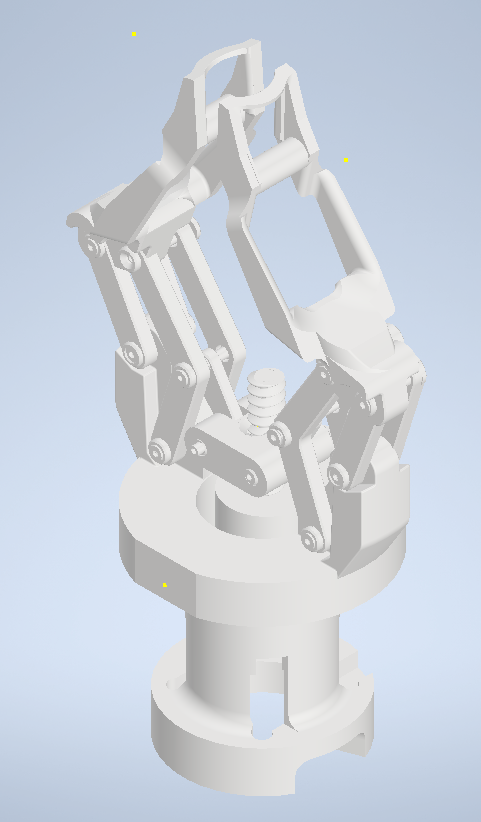
\includegraphics[width=\linewidth]{Pictures/Assembly_gripper.png}
        \caption{Assembly of the gripper}
        \label{fig:Gripper-Assembly}
    \end{subfigure}
    \hspace{0.01\linewidth}
    \begin{subfigure}[t]{0.27\linewidth}
        \centering
        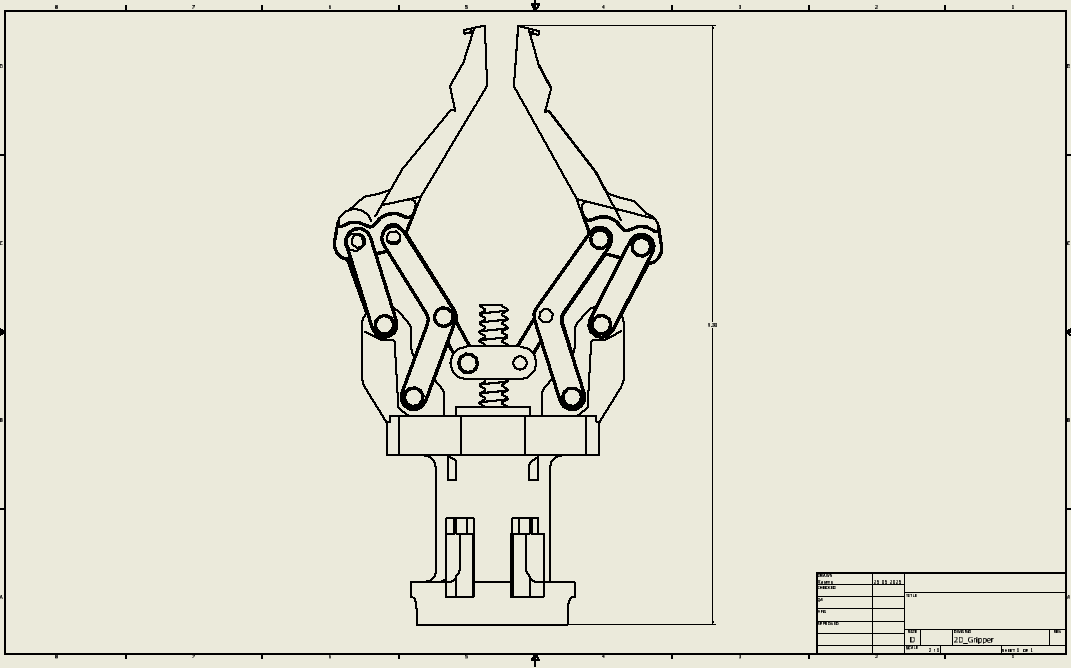
\includegraphics[width=\linewidth]{Pictures/2D_Gripper.png}
        \caption{2D drawing of the gripper}
        \label{fig:2D_Gripper}
    \end{subfigure}
    \hspace{0.01\linewidth}
    \begin{subfigure}[t]{0.22\linewidth}
        \centering
        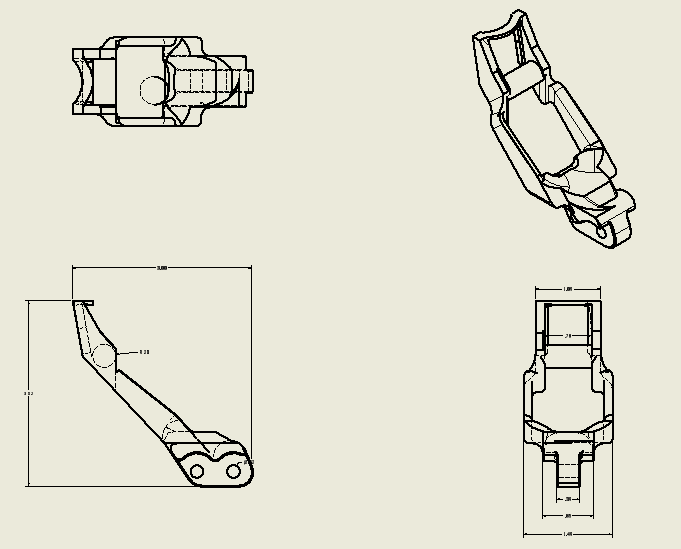
\includegraphics[width=\linewidth]{Pictures/Finger_plates_2D.png}
        \caption{2D drawing of the finger plates}
        \label{fig:2D_Finger_plates}
    \end{subfigure}
    \hspace{0.01\linewidth}
    \begin{subfigure}[t]{0.27\linewidth}
        \centering
        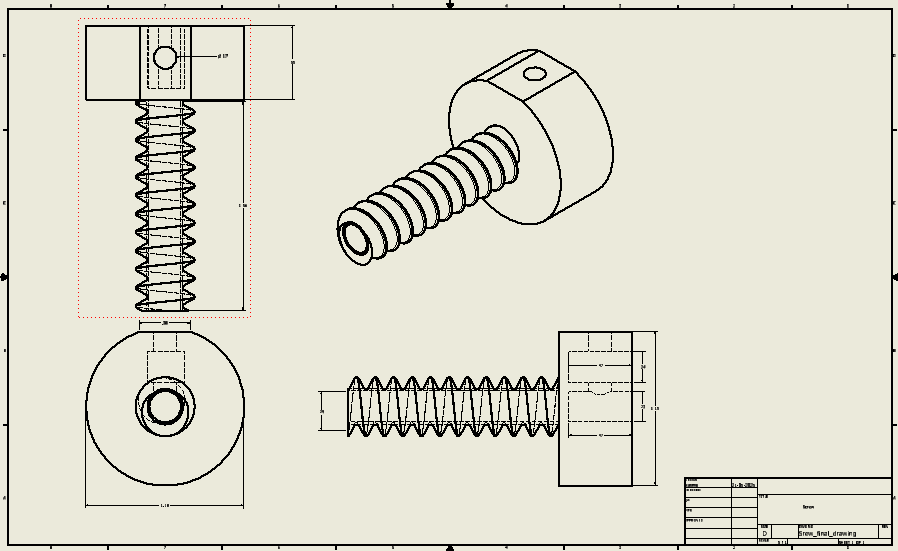
\includegraphics[width=\linewidth]{Pictures/Screw_drawing.png}
        \caption{2D drawing of the screw}
        \label{fig:Screw_drawing}
    \end{subfigure}
    \caption{Overview of the gripper design and drawings}
    \label{fig:GripperOverview}
\end{figure}

On the DC-motor there is a 3D-printed screw which is attached with a nut and a bolt to make sure it stays tight. When the DC-motor turns, it spins the screw around and pushes the 3D printed nut up and down, making a screw joint, which is connected to the gripper arms. This causes the two plates on the gripper to move in and out, which lets the gripper pick up the chess pieces. The two fingers are designed to fit the exact chess pieces used for the project, both in height and width.
In \cref{sec:ChessSpecs} these specifications are described. As the width varied from 16 mm to 19 mm the distance between the tips therefore needs to be smaller than 16 mm when closed.
Therefore when the gripper is closed the tip creates an ellipse with one semi-axis of 8 mm and the other of 19.5 mm. When the gripper then squeezes the piece, the tip latches onto the piece's indent and secures it. In addition to the latch mechanism, the finger also has a hollowed-out design, which provides a hole for neighbouring pieces.

The gripper is attached to the UR robot with 4 M6 screws. 

\subsection{Control}
By turning a DC motor clockwise or counter-clockwise, the gripper can be opened or closed. To accomplish this, a Pico is used to control when the gripper should close, open, or stand by. To turn the motor in both directions, an H-bridge is designed and used for bidirectional current, which can be seen in \cref{fig: Complete schematic}. 

\begin{figure} [H]
    \centering
    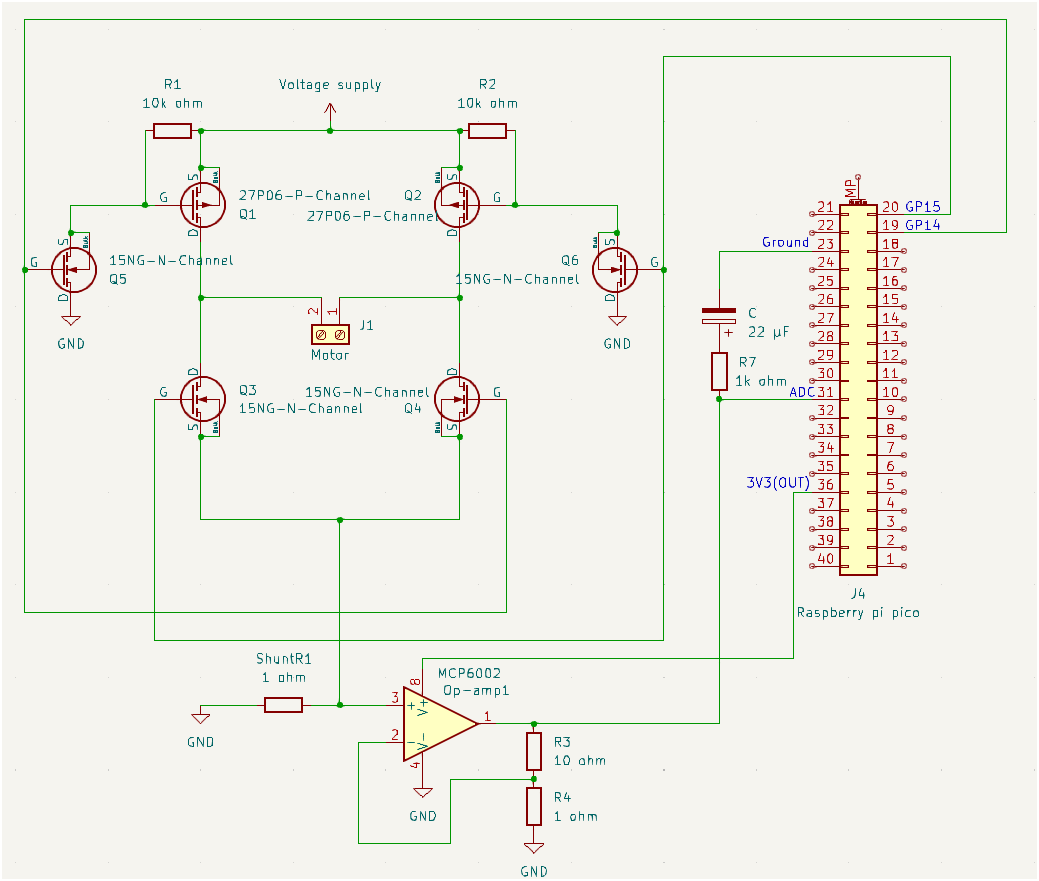
\includegraphics[width=0.8\linewidth]{Pictures/Complete_schematic.png}
    \caption{Schematic of the H-bridge, shunt resistor, low-pass filter and amplifier all connected.}
    \label{fig: Complete schematic}
\end{figure}

The H-bridge uses six transistors to control the direction of the current. 4 n-channel MOSFETs (metal-oxide-semiconductor field-effect transistors) and 2 p-channel MOSFETs are used in the design of the H-bridge. The n-channel MOSFETs used are 15NG \cite{15NG} and the p-channel are 27P06 \cite{27P06}.The 2 transistors Q5 and Q6 are used to control which direction the current runs. When the transistors are closed, no current runs, meaning the voltage across Q1 and Q2 gates, are the supply voltages, and the transistors are therefore closed. When Q5 is opened current runs from the source, though R1 and the transistor Q5. This results in a voltage of $0 \text{V}$ on the Q1 gate, and it therefore opens. The gate on Q5 and Q4 are connected and Q4 is therefore also open. The current can then run through the motor. The same applies when opening Q6 and Q3 to make the current run the opposite way.

To determine when the gripper is closed, a shunt resistor is put in series with the motor and an ADC pin on the Pico is used to read the voltage over the shunt resistor. For the shunt resistor to have as little effect on the rest of the circuit, the resistance needs to be low and therefore needs to have a low resistance. A resistor of 1 $\Omega$ is therefore used. 

The voltage over the resistor varies based on the current running through. The current is determined by the resistance of the shunt resistor and motor. The resistance in a motor is called inductive resistance. A DC motor has a low inductive resistance, when starting, stopping, or is blocked, which leads to an increase in current. The increase in current results in an increase in voltage. This increase happens due to "back EMF" (electromotive force) \cite{Back_EMF}, which is generated while the motor is running. Back EMF is voltage generated when the motor rotates. This voltage counteracts the voltage over the motor. This happens because of electric inductance. The state of the motor can therefore be found by measuring the voltage over the shunt resistor.

Making the shunt resistor have a small resistance results in small voltages drops over the resistor, which is hard to read by the ADC on the Pico. An op-amp as an amplifier is therefore used to amplify the voltage by $\frac{1 \Omega + 10 \Omega}{1 \Omega}=11$ times. 
The op-amp being used is MCP6002 \cite{MCP6002}.
When closing the gripper, a plot of the read ADC values can be seen in \cref{fig: ADC graph without capacitor}
The friction in the gripper results in the current having noise, and therefore the voltage read has noise.
A low-pass filter is placed to compensate for the noise generated. This is important since the ADC values should not accidentally exceed the threshold before the gripper is closed.

\begin{figure}[H]
    \centering
    \begin{subfigure}[t]{0.49\linewidth}
        \centering
        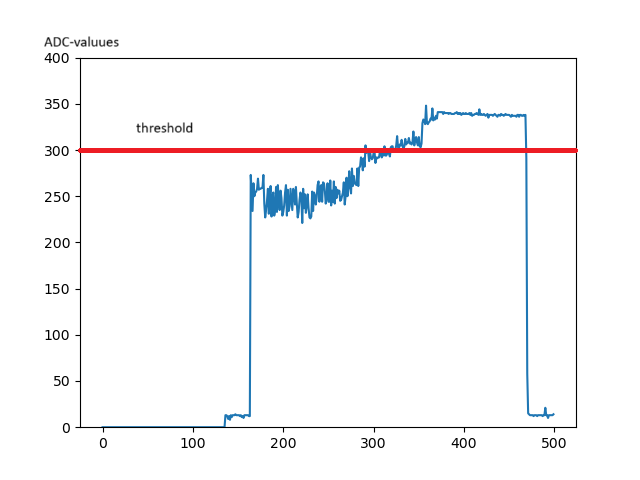
\includegraphics[width=0.8\linewidth]{Pictures/Billede af graf UDEN lavpasfilter.png}
        \caption{Graph over ADC values without a low pass filter.} 
        \label{fig: ADC graph without capacitor}
    \end{subfigure}
    \begin{subfigure}[t]{0.49\linewidth}
        \centering
        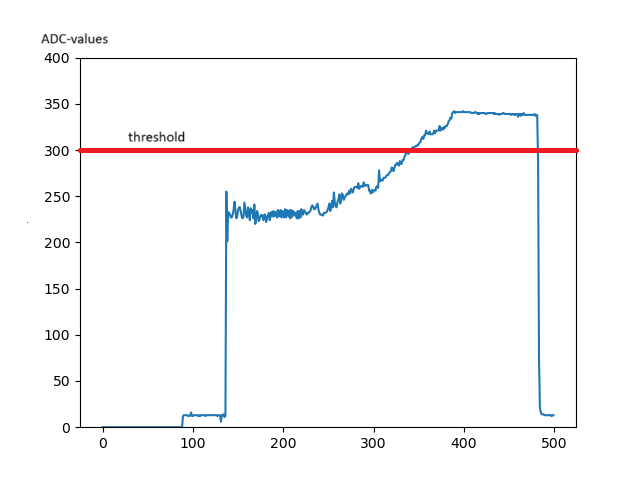
\includegraphics[width=0.8\linewidth]{Pictures/Billede af graf med lavpasfilter.png}
        \caption{Graph over ADC values with a low pass filter.}
        \label{fig: ADC graph with capacitor}
    \end{subfigure}
    \caption{Graph read from ADC with, a low pass filter, and without}
\end{figure}

Through analysing the ADC values which is shown on \cref{fig: ADC graph with capacitor}, the cut-off threshold is set to 300 corresponding to the value by the 12 bit ADC and corresponds to a voltage of $\frac{300}{4096} \cdot 3.3 \text{V} = 0.2417 \text{V}$.
When opening the gripper, the motor is just turned on for 11 seconds, which was found experimentally to be suitable.



\subsection{Communication}
To determine when to open or close the gripper, the Pico must communicate with the rest of the program. This is done with serial communication though the USB. 
 
The serial communication between the host computer and the Pico is full-duplex, allowing simultaneous data transmission and reception between them. The serial port is opened using the standard c libary fcntl. \cite{fcntl} The specification of the communication can then be configured using another standard c libary, termios, which has a struct to configure the communication protocol.

A baud and data-bit format is configured for the communication to be 115200 and 8-bit respectively, which defines how fast the data is transmitted and structured over the serial line. This ensures that data is not misread or lost. The Pico sends integers from the ADC values from the shunt resistor to the host computer. 
The host computer reads the ADC values and communicates with the Pico whether it should standby, close or open the gripper. This protocol can be seen in \cref{fig: Communication_Pico}

\begin{figure} [H]
    \centering
    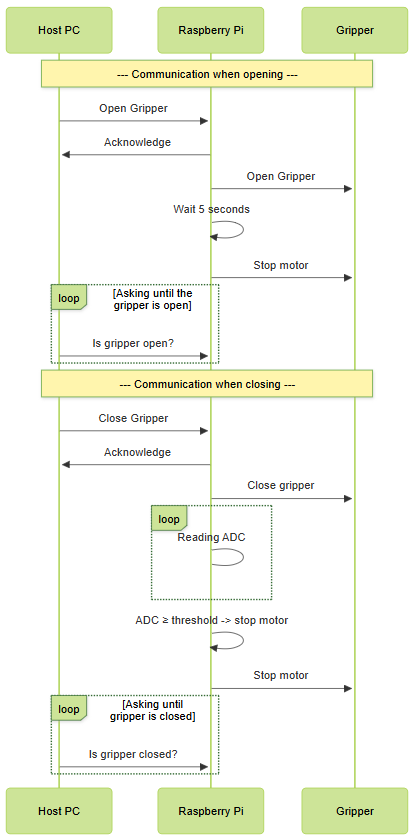
\includegraphics[width=0.5\linewidth]{Pictures/Sequence_Com_Pico_PC.png}
    \caption{Communication between Pico and host PC}
    \label{fig: Communication_Pico}
\end{figure}

